% !TEX root = ../../main.tex
% !TEX spellcheck = en_US
\section{Squads}
A squad, in BATS, are units grouped together acting in coordination. All squads have the abstract Squad class as their base class. 

\paragraph{Creating, deleting, and retrieving squads}
The squad manager updates and removing existing squads (but only from the squad manager); any class can create a squad and it adds itself automatically to the squad manager (via the squad's constructor). The squads are added as \texttt{shared\_ptr}, meaning they are automatically destroyed when no more references exist, i.e. no memory leaks. When a squad holds no units—achieved when all units died, units moved to another squad, or the squad disbands—the squad manager automatically removes it; but it can still be used if another class saved it before it was removed. Removed Squads have to be recreated to be inserted into the squad manager again.

Squads can be retrieved using two (actually four) different functions, either by the squad's id (automatically set) or by squad type (template function), shown in listing \ref{lst:SquadManager::getSquads()}. The template function will also return all sub-classes to the specified class, meaning \texttt{getSquads<AttackSquad>();} would return both Attack squads and Drop squads because Drop squad derives form Attack squad. The last two functions are there for convenience, the first returns the current frontal attack (if one exist), and the other returns all distracting attacks.
\begin{lstlisting}[caption={Template function to retrieve squads of the specified type},label={lst:SquadManager::getSquads()}]
template <typename T>
vector<shared_ptr<T>> SquadManager::getSquads();
\end{lstlisting}

\subsection{Squad base class}
Only the core functions of the squad base class are covered below, as there are too many helper functions to cover them all. If the reader wants to find out more information about the internal structure of the squads, s/he can look in Appendix \ref{sec:doxygen}. Squad movement will be covered first, then the squad's basic behaviors, which can be overridden by derived classes; and finally how the \texttt{update()} and \texttt{updateDerived()} functions work.

\paragraph{Squad movement}
This is not the specific unit movement, but where the squad's units move to. The potential field manager takes care of how units move and was already implemented in BTHAI\cite{bthai}—although some minor changes have been made to the potential field manager to accept some general squad behavior, more specifically moving towards the retreat location when retreating and when close to enemies. The squad has five prioritized locations it can move to. Starting from the lowest priority is
\begin{enumerate}
	\item The goal location where the squad want to go to do their main task (e.g. scout, attack, defend location).
	\item A retreat location to be able to retreat from e.g. an attack; there is no automatic retreat behavior in the base class, derived squads has to set the retreat location and the base class calls \texttt{onRetreatCompleted()} when the retreat succeeds or fails.
	\item To move to either the goal or retreat location a via path, that holds with multiple locations, can be used. Useful when attacking or retreating with a drop to make it move along the map's edges so that it does not run straight through the enemy.
	\item Temporary goal location, used when derived classes need an additional goal location, such as \nameref{sec:attack_squad}s waiting in a location to attack or \nameref{sec:hold_squad}s moving from their roaming area to the defended area when an enemy enters the defend perimeter. The temporary goal location is, however, disabled when a retreat location is active.
	\item Regroup location, the regroup is automatically handled by the squad when units are too spread out—a unit is further away than \squadRegroupDistanceBegin from the squad's center, the regroup stops again when all units are within \squadRegroupDistanceEnd. The squad will regroup to the unit who is closest to the goal position—first the squad's center was used but this caused units in the front to move backward and did not work very well, in addition the squad movement felt weird as if BATS could not decide what it wanted. Bugs can still occur when moving around a C shaped cliff as units to the left of the C are further away then those at the bottom location, if the goal is to the right of C. The regroup functionality can be disabled by derived classes, useful when sending reinforcements to the squad.
\end{enumerate}

\paragraph{Behaviors}
The squad has four elements that can change the behavior of the squad.
\begin{description}
	\item[Regrouping] which has been fully described above in squad movement.
	\item[Retreating]. While the base class squad never uses this directly, derived classes can set a retreat location and the squad will then check when it is close to the retreat location. Once close it will call \texttt{onRetreatCompleted()} which has the default behavior of disbanding the squad, thus merging it with the Patrol squad. By overriding this function another behavior can be accomplished. Retreat locations are most commonly retrieved from \nameref{sec:defense_manager} via the \texttt{findRetreatPosition()}, if a squad uses another location this will be mentioned.
	\item[Unit composition] a unit composition limits the squad to only contain units of the specific type, useful when creating special type of squads. Section \ref{sec:unit_composition} describes unit composition in more detail.
	\item[Avoid enemies] Some squads do not want to get close to enemies, in this case avoid enemies can be turned on. This causes attacking units to move to a specific location without attacking while trying to avoid enemies, this works most of the time but not always; the potential field manager in BTHAI did not support this behavior entirely as it needs to check that the unit retreats in the right direction, this was slightly improved by adding the goal location to the potential field calculation when avoid enemies is set, the calculation of goal location was already implemented but not used in BTHAI.
	\item[Wait goals] has been mentioned earlier in section \ref{sec:attack_coordinator} \nameref{sec:attack_coordinator} and is fully described in section \ref{sec:wait_goals} \nameref{sec:wait_goals}. While adding these does not give the base squad any specific behavior, they can be used in the derived classes for trigger behaviors.
\end{description}

\subsection{Attack squad}
\label{sec:attack_squad} The Attack squad can both function on its own, but is also the base class
for all attacks—in the current version only drops derives Attack squad. Used alone, it can either do
a regular attack or follow a teammate squad—a regular attack or battle in this section is a synonym
for an attack or battle where it not follows a teammate squad.

For regular attacks the squad requests an attack from \nameref{sec:attack_coordinator} to get an
attack location to move to and regroup when needed. When the squad is close to the attack location
(\squadAttackWaitingPositionDistanceFromGoal), i.e. its wait location, it will wait here until all
its Wait goals are finished, then it will continue moving to its attack goal. This will sync the
attack with other attacking squads as they wait until the squad either is in the wait location,
under attack, or already attacking.

If it encounters any enemies on the road it will try to kill them, unless they are too strong where
the squad will retreat instead; the squad can decide to retreat from any regular battle at any time,
depending on the situation. For an attack to succeed with its mission all structures within the
radius of \squadAttackStructuresDestroyedGoalDistance from the attack location needs to be
destroyed. After succeeding with the mission the squad will retreat back to the base, disband the
squad, and merge with the \nameref{sec:patrol_squad}.

\paragraph{Following a teammate squad}
To follow a teammate squad it can either be set directly when creating the Attack squad or later by
a call to \texttt{followTeammateSquad(teammateSquad)}, this converts the regular attack to follow
the specified squad—Attack squads can only convert to following a teammate and not from.


\begin{lstlisting}[caption={Squad actions depending on the teammate squad's state},label={lst:attack_follow_allied}]
switch (mTeammateSquad->getState()) {
	// Regroup if not close
	case IdleOutsideBase:
		handleTeammateRegrouping();
		setAvoidEnemyUnits(true);
		break;
	
	// Go to teammate target location, don't attack
	case Retreating:
		if (isRegroupingWithTeammate()) {
			clearTeammateRegrouping();
		}
		setGoalPosition(mTeammateSquad->getTargetPosition());
		setAvoidEnemyUnits(true);
		break;

	// Go to target location, attack if see anything
	case MovingToAttack: 
		if (isRegroupingWithTeammate()) {
			clearTeammateRegrouping();
		}
		setGoalPosition(mTeammateSquad->getTargetPosition());
		setAvoidEnemyUnits(false);
		break;

	// Find something close to attack
	case Attacking:
		handleTeammateRegrouping();
		if (!isRegroupingWithTeammate()) {
			setAvoidEnemies(false);
			msAttackCoordinator->requestAttack(this);
		}
		break;

	// Retreat, then merge with Patrol Squad (disband)
	case IdleInBase:
		setRetreatPosition(mpsDefenseManager->findRetreatPosition());
		mTeammateSquad.reset();
		break;
}
\end{lstlisting}
When the squad follows an teammate squad it behaves differently, depending on the teammate squad's
current state, described below in listing \ref{lst:attack_follow_allied}.

While most of the code speaks for itself, some functions need extra clarification.
\texttt{handleTeammateRegrouping()} checks if the distance to the teammate squad becomes to large
(\squadAttackAlliedRegroupBegin), it both sets the regrouping location to the teammate's center
location and the squad to avoid enemy units—the regrouping is considered done when the distance
between the squads are less or equal to \squadAttackAlliedRegroupEnd~away.
\texttt{setGoalPosition(mTeammateSquad->getTargetPosition())} sets the squad to move to the location
where most of the teammate squad's units are moving to; thus it will meet up with the teammate's
squad around that location. If handleTeammateRegrouping() was used it would try to chase after the
squads current location—much like in football (soccer) you shall run where the ball is heading and
not where its current location. This also allows the teammate to control where the bot shall attack
as it will attack where the player decides to attack.

\texttt{mpsAttackCoordinator->requestAttack(this)} uses \nameref{sec:attack_coordinator} to find a place to attack; as mentioned in section \ref{sec:attack_coordinator} it will find an attack location close to the teammate squad's target. Why not use the target as with MovingToAttack and have the AttackSquad create the attack location? Because
\begin{inparaenum}[1\upshape)]
	\item we want all attack request to be in the same location, if the attacks needs to be fixed or better coordinated we only need to change it in one place;
	\item in the future the squad could get a location of a prioritized building to attack; and
	\item using teammate target directly it will cause our units to fight exactly where the player is, which might crowd the place not making all units able to fight, but could be better if squads are smaller—more experimentation on this subject is needed.
\end{inparaenum}

In addition the squad need to cope with when the teammate squad splits or merges with another teammate squad. If the current teammate squad is empty of units (as it can become when it merges with another teammate squad) it will search for close (\squadAttackFindAlliedSquadDistance) teammate squads and follow the largest squad. If no teammate squads were found, it will retreat and then disband.

\subsection{Drop squad}
\label{sec:drop_squad}
A Drop squad is an attack containing a flying transportations along with some offensive units it
carries. The goal of the drop is to attack the enemy base from an undefended angle (as flying units
can fly over all terrain). In ideal situations the drop will unload its units and destroy either
significant bases or workers, but the goal is rather to distract the enemy for various reasons—e.g.
expanding and we do not want the enemy to attack, or the dropping player will attack from another
location simultaneously.

The Drop squad uses Attack squad as its base class. Listing \ref{lst:drop_squad} shows the behavior of the squad.

\clearpage
\begin{lstlisting}[caption={Drop squad behavior},label={lst:drop_squad}]
switch(mState) {
case LoadUnits:
	if (isTransportDoneLoading()) {
		setState(Transport);
	}
	// Note, no break!

case Transport:
	// travelsByGround() = cannot load all units
	if (travelsByGround() && !isRetreating()) {
		setState(Attack);
	} else if (isEnemyAttackUnitsWithinSight()) {
		if (isEnemyFasterThanTransport()) {
			setState(Attack);
	} else {
		if (!hasWaitGoals() && isTransportInGoalRegion()) {
			setState(Attack);
		}
	}
	break;

case Attack:
	// If we cannot load all units, don't load
	if (travelsByGround()) {
		break;
	}

	// Retreat when enemy units arrive, unless they are faster than us
	if (isEnemyAttackUnitsWithingSight()) {
		if (!isEnemyFasterThanTransport()) {
			setState(LoadUnits);
		}
	}
	// No enemies within sight, load if we aren't in the goal region
	else {
		if (!isTransportInGoalRegion()) {
			setState(LoadUnits);
		}
	}
	break;
}
\end{lstlisting}
While the code explains it self, setState() does not, as it changes the behavior of the squad. \texttt{setState(LoadUnits)} loads all ground units and disables regrouping; \texttt{setState(Transport)} enables regrouping again; and \texttt{setState(Attack)} sets the transportation to unload all units and enables regrouping.

The Drop squad uses the same method as Attack squad to check if its goal has completed, although it rarely does. Because the goal of the drop is not to destroy all buildings, merely to distract the enemy, it also has a timeout function which will make the drop retreat after \squadDropAttackTimeout, but only if it's not currently in the target region.

Now you know how it works, but which units will be used for the drop, as drops should not just use
random units and hope for the best? It uses \nameref{sec:unit_composition}s for this—section
\ref{sec:unit_composition} describes the unit composition and the drop's unit compositions, i.e. all
available squads, can be found in listing \ref{lst:unit_comp_drop}. 



\paragraph{Drop squad movement}
The target location to drop is, as mentioned, required by the attack coordinator, but the transport does not move in a direct path to the location (once the units are loaded), instead it will move along the edge of the map illustrated in figure \ref{fig:drop_squad_movement}.
\begin{figure}[htb]
\centering
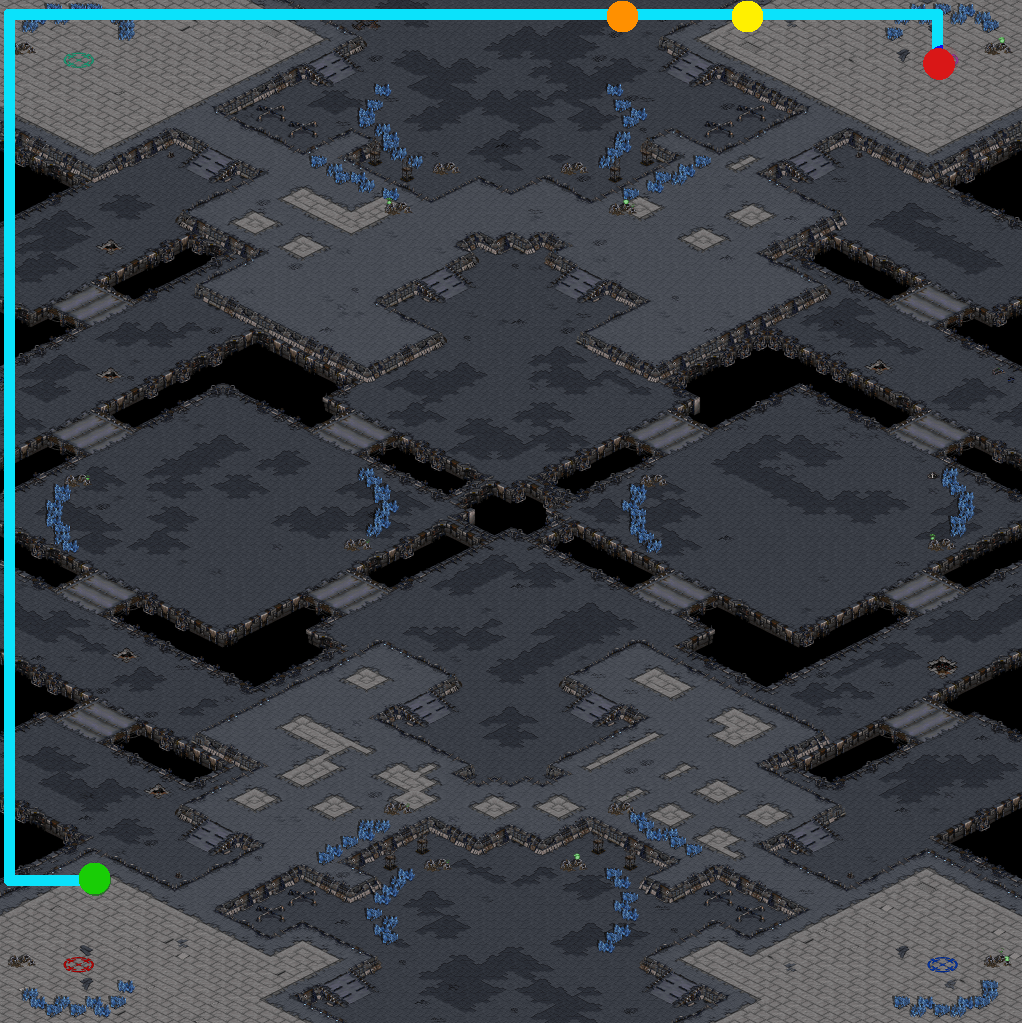
\includegraphics[width=0.75\textwidth]{space_atoll_(co-op)_drop_path}
\caption[Drop squad movement example]{Example of Drop squad movement.
\usebox{\LegendDotGreen}~Start location where the transportation loads the units.
\usebox{\LegendLineCyan}~Path to the drop target.
\usebox{\LegendDotOrange}Squad waits here, if it has Wait goals.
\usebox{\LegendDotYellow}Where the squad starts to unload.
\usebox{\LegendDotRed}Target location to attack.}
\label{fig:drop_squad_movement}
\end{figure}

\subsection{Patrol squad}
\label{sec:patrol_squad}
Patrols units between a set of locations, in the current version of BATS it only patrols between our defend positions which the \nameref{sec:defense_manager} takes care of. The units in the squad automatically attacks close enemies, but all units will not go to that location; instead another manager needs to tell the defensive squad what to do, e.g. the Defense manager will tell the squad where to defend. The squad will move to the defended area and attack all units within the defend perimeter (\squadDefendDefendPerimeter), but will remain in the defended area until no enemy units are within the enemy offensive perimeter (\squadDefendEnemyOffensivePerimeter).

The Patrol squad will never succeed with its goal, as the goal is to patrol between the specified locations the entire game— although the locations usually change during the game.

\subsection{Hold squad}
\label{sec:hold_squad}
The Hold squad has one goal, to hold a location from enemies; any location could be held, but it is designed to hold choke points. The squad contains a hold location and a roam location. The hold location works in more or less the same way as Patrol squad's defense location, i.e. if enemy units enter the defend perimeter (\squadDefendDefendPerimeter~in radius) it will move and attack those units, as the squad always will defend here it does not bother checking if enemies are within the enemy offensive perimeter as the Patrol squad does. The roam perimeter (\squadDefendRoamPerimeter~in radius) is where the units in the squad will move to and stay until enemy units move within the defensive perimeter.

Terran siege tanks have a special ability when their are in this squad and the bot has researched the siege mode ability. The siege tank will automatically siege up in the roaming area effectively defending the hold perimeter (and other close positions) from its location.

Hold squads use \nameref{sec:unit_composition}s to know which units should be in the Hold squad—section \ref{sec:unit_composition} describes unit compositions in general and listing \ref{lst:unit_comp_defend} shows the composition file used for Hold squads. The current unit compositions used by BATS are listed below; the top is the composition with least priority, whereas the bottom is the one with highest priority. The name of the composition is in bold text.

\begin{function_description}
	\item[Marine spotter] 1 Marine
	\item[Bunker Marines] 4 Marines
	\item[Marine Medics] 4 Marines, 1 Medic
	\item[Tanks 1] 1 Siege tank
	\item[Tanks 2] 2 Siege tanks
	\item[Tanks 4] 4 Siege tanks
\end{function_description}
The Marine spotter is used to watch for enemies as one marine alone is not a good defender. Bunker marines are used for bunker, this strategy does not work with the current version of BATS as one cannot bind a Hold squad to a specific location where there for example is a bunker. Marines and medics generally make a good composition, but these number are too low to hold of almost any attack, but they can still delay the attack until reinforcements can arrive, these are however not used in the experiment as none of the build orders build medics. Tanks are very good positional holders and can hold of almost anything coming through choke points\cite{day9}.

\subsection{Scout squad}
\label{sec:scout_squad}
Scouts regions and expansions that have not been scouted for a long time, to be exact it will always move to the region or expansion that our team visited the longest time ago. The \nameref{sec:exploration_manager} handles this and thus the Scout squad gets it target location from it. To avoid multiple scouts moving to the same location the scout location will set its last visit time when the squad gets the location, although it hasn't been visited at all.

When an enemy is seen close to the scout it will abandon its current scout location and find another one, the idea is to save the scout from being killed by the enemy. This, however, does not work correctly all times as the units will move away from the enemy and at the same time towards the goal, but if the new scout location happens to be on the other side of enemy the scout will just roam around the outer edge of the enemy. To be sure that the scout does not switch scout locations all the time when an enemy is present it will only switch once its close to any enemy, it will then need to get out of the range before it can switch goal again.

\paragraph{Further optimizations}
When another unit visits the target location the squad will not complete its goal until it has reached there itself. Currently the squad moves from one end of the map to the other (already passing recently scouted areas), an improvement would be to either let the squad get regions and expansions that abut to its current location (or more correctly improve Exploration Manager), or search for the most optimal path (in regard to visit not-recently visited locations) when moving to the target location—i.e. use its via path. The first option is probably preferable as it is easy to calculate and easy to check if the first limitation should be solved, otherwise one must check all via paths and the path might not be the optimal anymore if one location is removed.

\subsection{Unit composition}
\label{sec:unit_composition}
In a nutshell, the unit composition is a feature for the squads to require specific types of units. E.g. Hold squads require specific unit groups (compositions) as was explained above in section \ref{sec:hold_squad}. All unit compositions used in bats can be seen in appendix \ref{sec:unit_compositons_in_bats}. The unit composition has two important elements: The priority and the units, higher value means higher priority, the units for the composition are listed under the units sub-section.

To use compositions one calls the unit composition factory which takes a composition type (hold-squad, drop, etc.) of and a list of units (usually free units). The unit composition factory will check which compositions can be created with the available units—the composition needs to be full—and then return these sorted by priority. It is then up to the caller of unit composition factory to decide which composition to use—for Hold squads it will always use the one with highest priority, drops on the other hand takes a random one.

\subsection{Wait goals}
\label{sec:wait_goals}
Wait goals were created for simple one time trigger abilities. These can be added to any squad at the moment, but will only have an effect on the squad if the derived squad handles them, as the squad base class only checks if the Wait goal has succeeded, failed, or timed out and send an event to the derived class.

To be updated Wait goals shall be added to the Wait goal manager which updates the goals, completed goals (succeeded, failed, timed out) will automatically be removed from the Wait goal manager. When adding an Wait goal to the manager an optional set type can be set, this allows all Wait goals with the same set type to be easily extracted—\nameref{sec:attack_coordinator} uses this when adding existing Wait goals to a new Attack squad.

\paragraph{Existing Wait goals}
For now there is only one type of Wait goal, WaitReadySquad. \nameref{sec:attack_squad}s uses these, as described in section \ref{sec:attack_squad}, to synchronize all its attacks—i.e. to attack the enemy simultaneously from different locations. The Wait goal will complete when the Attack squad is in position, \squadAttackWaitingPositionDistanceFromGoal from the attack location, when the squad is under attack or attacks, or if the Wait goal times out (\attackCoordinatorWaitGoalTimeout).
